\chapter{Research Questions and Methodology}
\label{ch:Research}
The long-term goal of my research is to improve the consistency of empirical evaluation research on low-level software processes. As a step in this direction, I designed and developed the Software Development Stream Analysis (SDSA) framework (Chapter \ref{ch:Framework}) that can infer development behaviors using automatically collected in-process software metrics. I used the SDSA framework to specify a low-level software process called Test-Driven Development (TDD) and implemented Zorro, a software system that can recognize development behaviors and measure the developer's process conformance to TDD. If Zorro, a specification of the SDSA framework, can be experimentally validated, I will have provided evidence that SDSA is an enabling technique for recognizing at least certain types of low-level development activities. 

In order to validate Zorro, I designed a series of case studies including a pilot study,a classroom case study and an industrial case study. The purpose of the pilot and classroom validation studies was to validate Zorro's data collection and TDD behavioral inference 
in controlled environments. The purpose of the industrial case study was to explore how Zorro can be used by external researchers. Section \ref{sec:Research-Questions} introduces the central research questions of my thesis research. Section \ref{sec:Research-Methods} presents my research methods including participant observation, interview and survey. 

\section{Research Questions}
\label{sec:Research-Questions}

\begin{comment}
If Zorro can correctly recognize development behaviors of TDD, 
then it can be used to assess process conformance during daily 
practice of TDD, as well as during empirical evaluation of TDD
to improve construct validity (see Chapter \ref{ch:RelatedWork} 
for details). However, does Zorro infer developers' TDD development
behaviors correctly? Will it falsely categorize some non-TDD
development behaviors as TDD? Or, will it misinterpret some TDD
development behaviors as non-TDD? To answer these questions, we 
need to conduct Zorro validation studies. 
\end{comment}

The central research questions of the Zorro validation studies were:
\begin{itemize}
\item Q1: Can Zorro automate the recognition of TDD behaviors
using automatically collected software metrics?  

This question can be further divided into three sub-questions:
   \begin{itemize}
     \item Can Zorro collect software metrics correctly?
     \item Does Zorro collect the necessary software metrics?
     \item Can Zorro infer TDD behaviors correctly based upon 
     automatically collected software metrics?
   \end{itemize}

\item Q2: How useful is Zorro? 

This question is hard to answer but it can be divided into three sub-questions based upon users' roles.

\begin{itemize}
\item For beginners, can Zorro help them improve their compliance to TDD?
\item For experienced TDD practitioners, will Zorro help them improve their TDD practice by providing them with new insight into their TDD development behaviors?
\item For researchers, can Zorro help them reach legitimate research conclusions on TDD experiments by providing them with TDD process conformance information?
\end{itemize}

\end{itemize}

\section{Research Methodology}
\label{sec:Research-Methods}

Answering the above research questions requires a ``mixed methods'' research methodology according to \cite{Creswell:03}. Question Q1 can be investigated using the participant observation. In order to investigate the research question Q2, we need to collect users' feedback or interview them. 

To use the participant observation method, we can observe participants in the field, take notes about their development activities and behaviors to provide an independent data source for validating Zorro's data collection and TDD behaviors inference. However, this manual participant observation method \cite{Creswell:03} does not work for studying low-level software development activities that could occur in seconds and minutes. It is simply too demanding for the observer to record all of the necessary information about a low level software process, where significant events can occur every few seconds. Thus, I developed a recording tool called ``Eclipse Screen Recorder'' (ESR) to assist participant observation. ESR is an Eclipse plugin that can generate a QuickTime movie containing time-stamped screen shots of the Eclipse window at regular intervals. With ESR, observers will not need to worry about missing rapid development activities. 

Figure \ref{fig:ESR} illustrates the Eclipse window with ESR installed. The two pictured buttons on the toolbar menu are defined by ESR. Pressing the green button can start the recording process and make the red button become enabled. The recorder will stop if either the red button is pressed or Eclipse is closed. 
\begin{figure}[htbp]
  \centering
  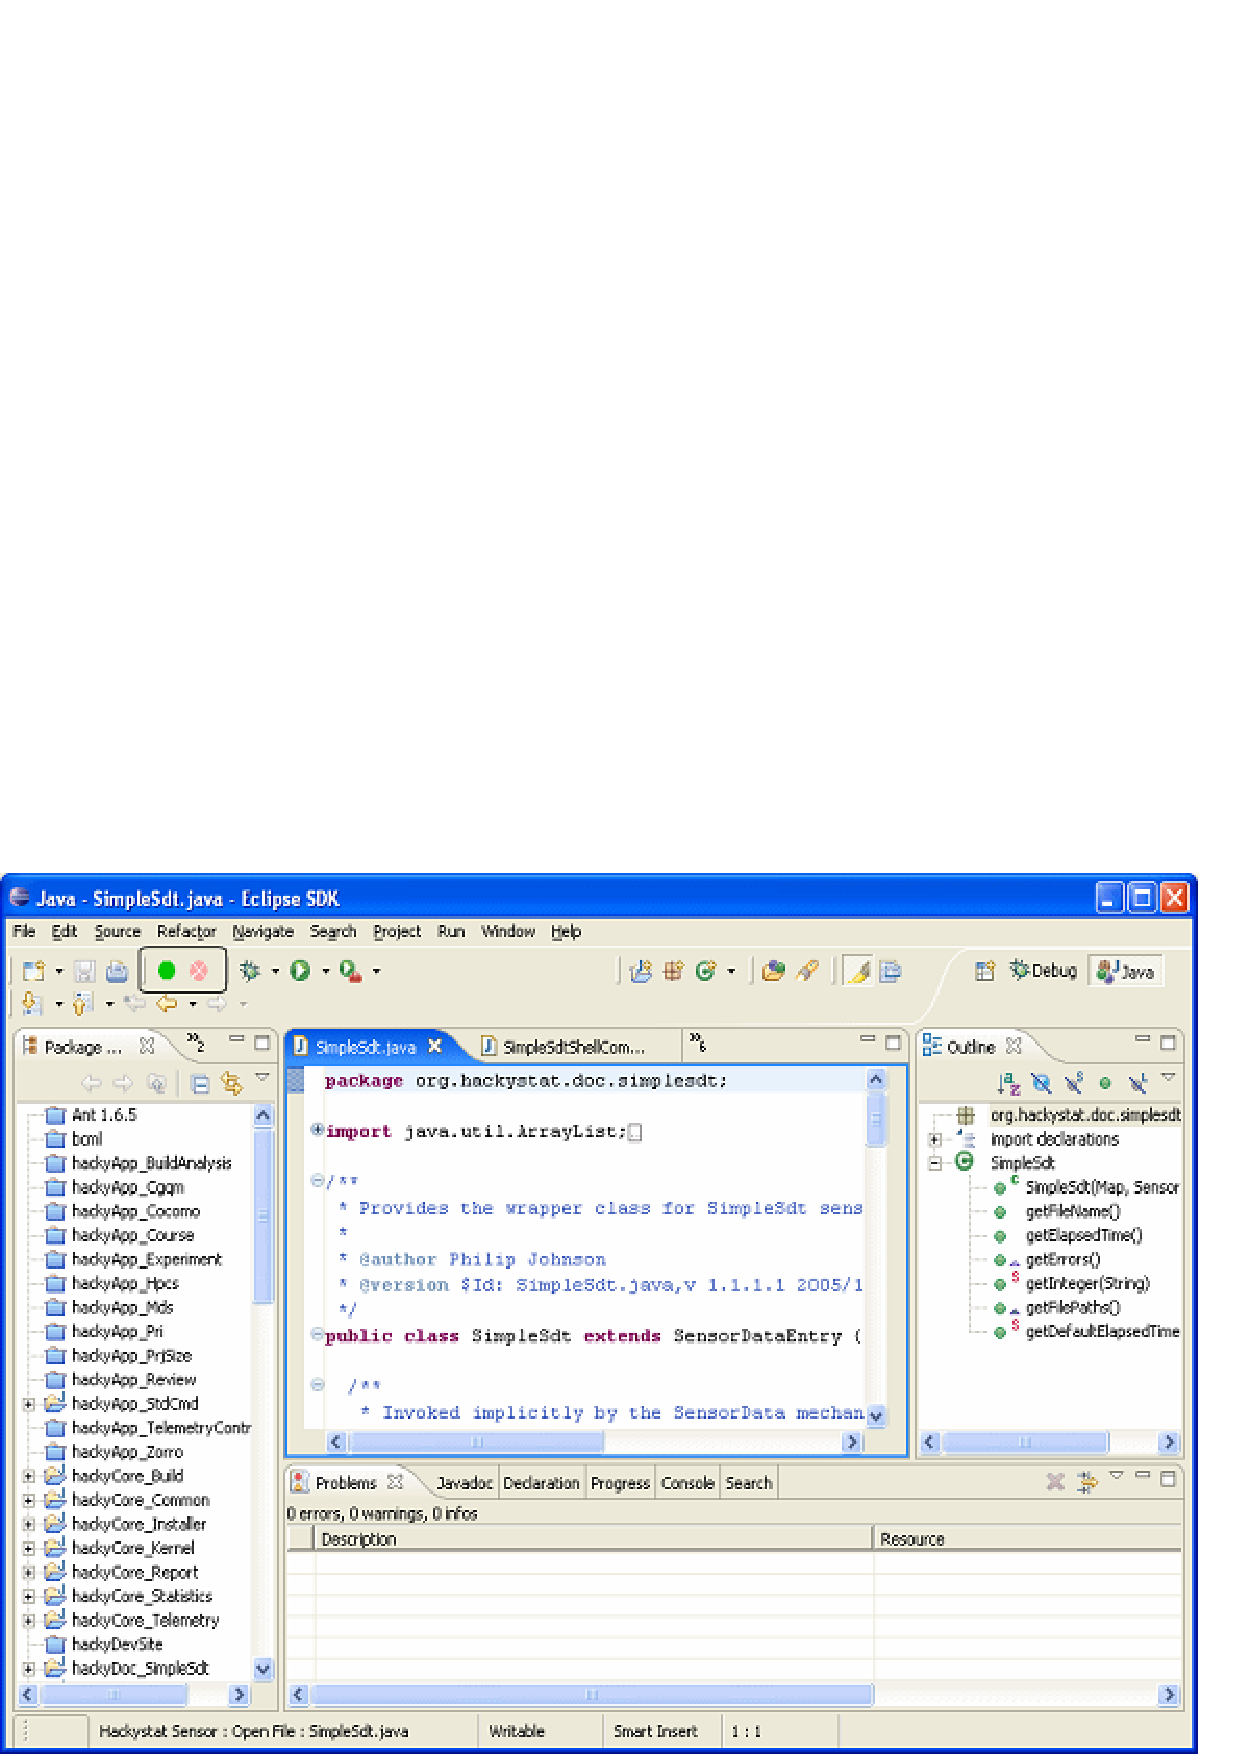
\includegraphics[width=0.8\textwidth]{figs/ESR}
  \caption{Eclipse Screen Recorder}
  \label{fig:ESR}
\end{figure}
Figure \ref{fig:ESR-Video} in Chapter \ref{ch:Introduction} illustrates the recorded movie being played by QuickTime. The embedded timeline at bottom of videos (See Figure \ref{fig:ESR-Video}) can be used to synchronize videos with development activities collected by Zorro for validation. ESR allows customization of recording rate (0.5-2 frames per second), picture quality, and resolution. One frame/second was found to be sufficient for validation, generating file sizes of approximately 7-8MB per hour of video. 

The development of Zorro was iterative and incremental. So was the validation of Zorro. I have conducted three case studies --- a pilot study, a classroom case study, and an industrial case study. Next, I will introduce the research methods I used in these case studies.

\subsection{Pilot Study}

I designed and implemented the Zorro software system based upon descriptions in books \cite{Beck:03,Astels:03,Newkirk:04,Link:03,Hunt:03} and my observation of TDD in practice. By Spring 2005, I had enhanced the Hackystat Eclipse sensor to collect necessary development activities, designed the SDSA  framework and implemented the Zorro software system to infer TDD development behaviors automatically. In the following Fall semester, I conducted a pilot Zorro validation case study.

The purpose of the pilot study was to test ESR as a tool to provide independent evidence for validating Zorro, as well as to validate Zorro's data collection and TDD behavior inference. The research method was participant observation using ESR as the data collection tool. I played recorded QuickTime videos to observe participants' TDD development activities and behaviors for Zorro validation. 

\begin{comment}
The specific research questions for the pilot study were:
\begin{itemize}
 \item Q1a: Does Zorro collect enough low-level development 
 activities to infer TDD behaviors?
 \item Q1b: Does Zorro's inference of TDD agree with analyses 
 based upon participant observation?
 \item Q1c: Is ESR a suitable tool for Zorro validation study?
\end{itemize}
\end{comment}


\subsection{Classroom Case Study}
The pilot study showed that participant observation with ESR is a suitable research method for conducting Zorro validation study. Though Zorro was not perfect at collecting necessary software metrics and inferring TDD behaviors, the pilot demonstrated that it was promising. Based on research results from the pilot study, I improved Zorro's data collection, enhanced Zorro's TDD behaviors inference, added heuristics on process conformance of TDD, and provided many TDD analyses and telemetry reducers (See Chapter \ref{ch:Zorro}). With these improvements, I conducted an extended validation study on Zorro in the software engineering classes at the University of Hawaii in Fall 2006. 

\begin{comment}
I addressed both of the research questions Q1 and Q2. The specific 
research questions for this study were:
\begin{itemize}
\item{Q2a: Does Zorro collect sufficient software development 
activities for episode partitioning and TDD behavior inference?}
\item{Q2b: Does Zorro's inference of TDD behaviors agree with
analyses based upon participant observation?}
\item{Q2c: Does Zorro's inference of TDD behaviors agree with what
participants believe to be their TDD behaviors?}
\item{Q2d: Does Zorro provide useful information for beginners to
understand TDD and improve their TDD development?}
\end{itemize}
\end{comment}

The purpose of the classroom case study was to validate Zorro in a controlled environment and investigate its usefulness for TDD beginners. The research method of the validation was also participant observation. Participants developed software using TDD in Eclipse with instrumentation including the Hackystat Eclipse sensor and ESR. ESR served as the data collection tool for participant observation and the recorded videos were analyzed to validate Zorro.

A caveat with the pilot study was that I, the author of the Zorro software system, analyzed the recorded videos for Zorro validation. This creates a ``construct validity'' threat with regard to this experiment design because ESR was the only source of evidence and my analysis could be biased. Therefore, in order to increase the construct validity of classroom case study, multiple sources of evidence were used according to suggestions from Yin in \cite{Yin:03} (Page 34). Participants' comments were the third source of information I used to cross-validate video analysis results. Prior to the study, I developed a Zorro validation wizard in web pages to let participants comment. 

To explore whether Zorro can help TDD beginners, I interviewed participants on their TDD development experiences. After the interview, each participant used the Zorro validation wizard to analyze his/her TDD development behaviors. Meanwhile, an embedded survey was conducted to evaluate Zorro's usefulness. To improve quality of the survey, I asked participants to justify their answers verbally. 

%to address the research question Q2d.

\subsection{Industry Case Study}
In Spring 2007, I conducted an industry case study to test Zorro's usefulness to TDD researchers. Using Zorro as a tool to assess TDD process conformance, Dr. Geir Hanssen and Dr. Tor Erlend F{\ae}gri from SINTEF ICT of Norway conducted a TDD vs. non-TDD comparison study in a Norwegian software company.

\begin{comment}
I focused on the research question Q2 to evaluate Zorro's usefulness
in this study. The specific questions were:
\begin{itemize}
\item Question Q3a: Can Zorro be deployed? 
\item Question Q3b: Does Zorro infer the TDD behaviors correctly as
participants' perception?
\item Question Q3c: Are Zorro's TDD analyses useful for participants?
\item Question Q3d: How can Zorro be used to assist TDD research?
\end{itemize}
\end{comment}

The purpose of this study was to explore how Zorro can be used by researchers to increase quality of TDD's evaluation research. I deployed Zorro in the software company, assisted the project manager and the researcher on analyzing process conformance data, and conducted a survey at the end of the study. 

% to address research questions Q3a-Q3d. 

\section{Chapter Summary}
This chapter introduced my research statement and Zorro's validation case studies. The central research questions were: (1) Can Zorro automate the recognition of TDD behaviors using automatically collected software metrics? and (2) How useful Zorro is?  To address these questions, I have conducted a pilot study, a classroom case study and an industry case study in which I used research methods such as participant observation, interviews and surveys. In order to improve the quality of data collection for participant observation, I developed ESR, a tool that can record the Eclipse window in high fidelity. Both the pilot study and the classroom case study used ESR as a data collection tool for Zorro validation. 

\begin{comment}

In Zorro, I converted the knowledge of TDD practice into a set of
rules to classify development behaviors of TDD on the development
stream consisting of automatically collected software metrics. 
So the software metrics that are related to TDD development 
behaviors must be collected, and the TDD inference rules must be 
correct. 

Thus, in order to validate Zorro, we need an independent
source that can oversee the low-level development activities of
TDD and 

a third party tool that can oversee the data collection process
and examine the inferred results. 


Beck literally introduced the 
development method of TDD in \cite{Beck:03}, which is the main resource
I used for 

Whether Zorro can automate the recognition of development behaviors of 
TDD relies on the capability of software metrics collection, as well as 
the correctness of inference rules. Thus, in order to validate Zorro,
we need an independent source of information of development activities
to compare to Zorro's. 

As a result, we can study process 
conformance using SDSA to improve the consistency of empirical 
research on low-level software processes. 

The long-term goal of my research is to understand how to characterize
and improve low-level software development behaviors.  As a step in
that direction, I am focusing for my Ph.D. research on a specific kind
of low-level software development behavior: Test-Driven
Development. The Zorro system, which attempts to infer TDD low-level
development behaviors, provides a way to partially evaluate the
overall approach and begin to understand its strengths and
limitations.

Zorro infers developer's TDD development behaviors using SDSA. It is
easy for software developers to collect in-process development
activities using Hackystat sensors, and it is also easy for them to
evaluate their TDD development behaviors using Zorro. If Zorro's TDD
inference is correct, then we can use it to assess TDD process
conformance during the daily practice of TDD as well as during empirical
studies of TDD. However, does Zorro infer developers' TDD development
behaviors correctly? Will it falsely categorize some non-TDD
development behaviors as TDD? Or, will it misinterpret some TDD
development behaviors as non-TDD? To answer these questions, we need 
to conduct validation studies of Zorro. Some of the most important research
questions are: 
\begin{itemize}
\item Q1: Can Zorro automate the recognition of Test-Driven Development
using automatically collected low-level software development activities?  
\item Q2: Can Zorro help to improve the practice of TDD? 

This is a hard question, but we can divide it into three small questions
with regard to user's roles.
   \begin{itemize}
   \item For beginners, can Zorro help them improve the compliance to TDD?
   \item For experienced TDD practitioners, will Zorro help them
   improve their TDD practice by analyzing their TDD development
   behaviors?
   \item For researchers, can Zorro help them reach legitimate
   research conclusions on TDD experiments by providing the TDD
   process conformance information.
   \end{itemize}
\end{itemize}

Answering these questions requires a ``mixed methods'' research strategy
\cite{Creswell:03}. Questions Q1 can be investigated by evaluating 
Zorro's data collection and TDD inference capability using field observation
research method. Investigating question Q2 requires research methods such  
as collecting users' feedback or interviewing them. In my research, 
I designed a series of case studies using these research methods to 
investigate the research questions I presented above.

\section{Evaluation Methods}
\label{sec:EvaluationMethods}
This chapter introduces three Zorro validation studies: a pilot study,
a case study with students from the software engineering class as
participants, and an external collaborative case study with the TDD
community of developers and researchers. Zorro uses low-level software
development activity data to infer developer's TDD behaviors.  In
order to validate its capabilities of data collection and TDD behavior
inference, a secondary data source must be used. In my dissertation
research, I will introduce two ways to provide the secondary data:
recording individual developer's TDD development process using the
Eclipse Screen Recorder (ESR) \cite{esr}; and gathering developer's
feedback to their TDD behavior inference results using the Zorro
validation wizard.  I have already used the ESR approach in the pilot
study. In the second case study, I will plan to use both approaches.

\end{comment}